%\documentclass[11pt]{article}

\documentclass[addpoints,10pt]{exam}

\usepackage[margin=2.5cm]{geometry}
\usepackage{graphicx}
\usepackage{listings}
\usepackage{xpatch}
\usepackage{color}

\makeatletter
\xpretocmd{\item@points@pageinfo}{\normalfont}{}{}
\xapptocmd{\item@points@pageinfo}{\bfseries}{}{}
\makeatother

\begin{document}
	\begin{center}
		\LARGE\scshape{Taller 1}
		
		\vspace{1cm}
		\large\scshape{Juan Barbosa - 201325901}
	\end{center}

	\begin{questions}
		{
			\question
			Medici\'on de la velocidad de filamentos de actina en \textit{glidding assay}
		}
				
		Para realizar la medici\'on se cargaron los datos usando:
		\begin{enumerate}
			\item \texttt{File > Open}
			\item \texttt{Analyze > Set Scale} (200 $\mu$m $\longrightarrow$ 512 px)
			\item \texttt{Image > Properties} ($dt = 0.14$)
			\item \texttt{Plugins > MTrackJ}
			\begin{enumerate}
				\item \texttt{Add} (Track 1)
				\item \texttt{Add} (Track 2)
				\item \texttt{Add} (Track 3)
				\item \texttt{Add} (Track 4)
				\item \texttt{Add} (Track 5)
				\item \texttt{Measure}
			\end{enumerate}
		\end{enumerate}
		
		\begin{figure}[h]
			\centering
			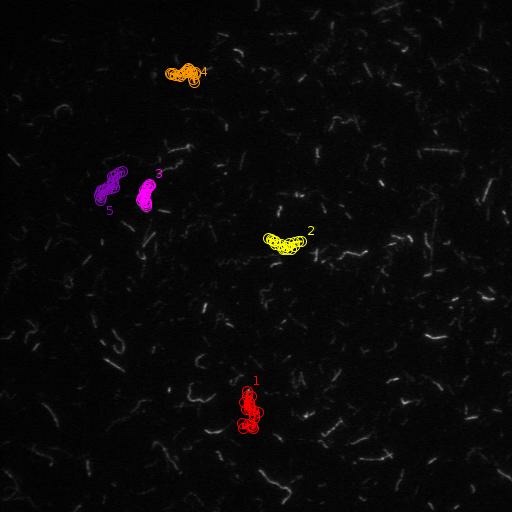
\includegraphics[width=0.35\linewidth]{trackimg.png}
		\end{figure}
		
		\input{p1table.txt}
		
		{\question Conteo de n\'ucleos}
		
		El conteo se llev\'o a cabo de la siguiente manera:
		\begin{enumerate}
			\item \texttt{File > Open}
			\item \texttt{Image > Type > 8-bit}
			\item \texttt{Image > Adjust > Threshold} (0, 45)
			\item \texttt{Process > Find Edges}
			\item \texttt{Analyze > Analyze Particles}
		\end{enumerate}
	
		\begin{figure}[h]
			\centering
			\begin{tabular}{cc}
				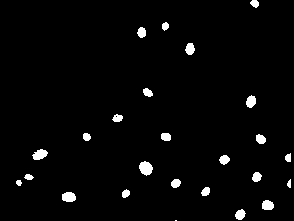
\includegraphics[width=0.35\linewidth]{threshold.png} & 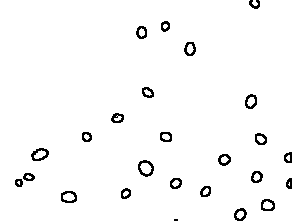
\includegraphics[width=0.35\linewidth]{edges.png}
			\end{tabular}
		\end{figure}
	
		\input{p2table.txt}
		
		Para automatizar este proceso se propone grabar la secuencia antes descrita usando macros.
		
		\lstinputlisting[basicstyle=\footnotesize, language=java, keywordstyle=\color{blue}]{Macro.ijm}
		
		{\question Reconstrucci\'on y tratamiento de im\'agenes 3D}
		\paragraph{Orthogonal views}
			Produce tres gr\'aficas, la principal contiene los ejes $XY$, la inferior $XZ$ y la derecha $ZY$. Lo anterior ver un punto definido en las tres dimensiones en los planos antes mencionados. 
			\begin{figure}[h]
				\centering
				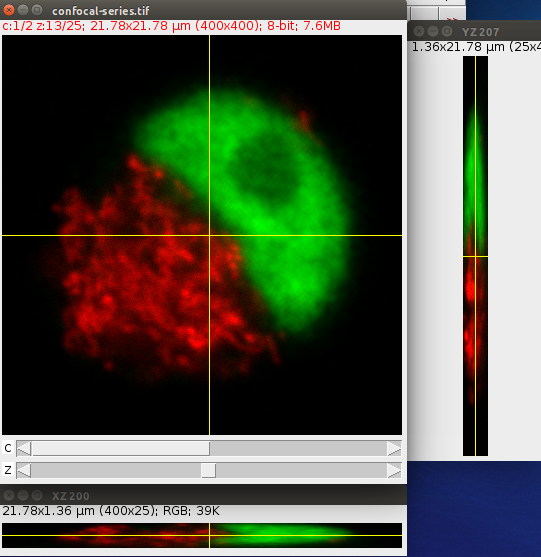
\includegraphics[width=0.5\linewidth]{ortogonales.png}
			\end{figure}
			
		\paragraph{Z project}
			Reduce las dimensiones de la imagen, se deja de tener un arreglo de varias im\'agenes a varias alturas por una sola en $z=0$. La informaci\'on con la que se construye esta proyecci\'on se puede variar, es posible tener encuenta todas las imagenes o solo unas cuantas. Adem\'as se debe especificar la operaci\'on a realizar sobre las im\'agenes: tomar el promedio de intensidades, m\'aximo o m\'inimo, suma, y desviaci\'on.
		
			\begin{figure}[h]
				\centering
				\begin{tabular}{cc}
					\includegraphics[width = 0.35\linewidth]{zproject.png} & 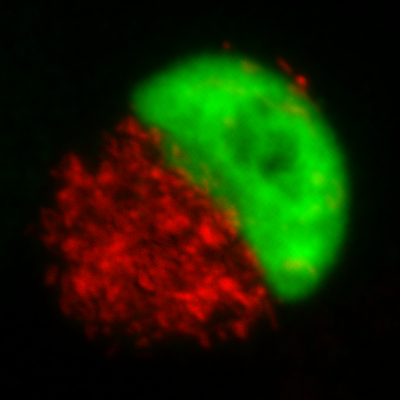
\includegraphics[width = 0.35\linewidth]{std.png}
				\end{tabular}
			\end{figure}
		{\question Problema abierto}
	\end{questions}
	
	
\end{document}
